% Nature Physics format manuscript
\documentclass[11pt]{article}

%%% Required packages
\usepackage[utf8]{inputenc}
\usepackage[T1]{fontenc}
\usepackage{graphicx}
\usepackage{amsmath,amssymb}
\usepackage{bm}
\usepackage{tikz}
\usepackage{pgfplots}
\pgfplotsset{compat=1.17}
\usepackage{booktabs}
\usepackage[colorlinks=true,linkcolor=blue,citecolor=blue,urlcolor=blue]{hyperref}
\usepackage[margin=2.5cm]{geometry}
\usepackage{xcolor}

% Nature-style superscript citations
\usepackage[super,comma,sort&compress]{natbib}

\begin{document}

\title{Spin chirality across quantum state copies detects hidden entanglement}

\author{Patrycja Tulewicz$^{1}$ and Karol Bartkiewicz$^{1,*}$}

\date{}

\maketitle

\noindent $^{1}$Institute of Spintronics and Quantum Information, Faculty of Physics, Adam Mickiewicz University, 61-614 Pozna\'n, Poland\\
\noindent $^{*}$e-mail: karol.bartkiewicz@amu.edu.pl

\vspace{1em}

\begin{abstract}
\noindent\textbf{Entanglement can hide in two fundamentally different ways: multi-copy correlations that no single-copy measurement on an unknown state can access, and bound entanglement that the Peres--Horodecki criterion cannot detect. Here we show that both forms emerge from the spectral structure of partial transpose moments, measurable via controlled-SWAP circuits with only three configurations for two-qubit systems. The moment decomposition uncovers multi-copy chirality---collective handedness patterns mathematically identical to the scalar spin chirality of topological condensed matter---providing a geometrically interpretable entanglement witness with zero false-positive rate for pure states. The same hardware detects bound entangled states through realignment matrix spectral features, correctly classifying all tested $3 \times 3$ states on four IBM Quantum processors with negativity mean errors of 0.002--0.027 and no misclassifications among all tested separable states.}
\end{abstract}

\vspace{2em}

Standard entanglement detection faces two structural blind spots. First, certain correlations between replicas of an unknown state cannot be expressed as expectation values of any single-copy observable $\mathrm{Tr}[O\rho]$\cite{PhysRevLett.89.127902,PhysRevLett.90.167901}---they are intrinsically multi-copy phenomena, invisible to all conventional measurements. Second, bound entangled states possess positive partial transpose\cite{Horodecki1998bound}, rendering them undetectable by the Peres--Horodecki criterion\cite{PhysRevLett.77.1413,HORODECKI19961} and the entire hierarchy of moment inequalities\cite{Yu2021optimal,Neven2021symmetry} that depend on it. These are two fundamentally different forms of hidden entanglement, yet they share a common origin: both reside in spectral structures accessible only through joint measurements on multiple state copies.

Partial transpose moments $\mu_k = \mathrm{Tr}[(\rho^{T_A})^k]$, measurable via controlled-SWAP circuits\cite{Travnicek2019,tulewicz2025} or randomized measurements\cite{Elben2020mixed,Huang2020shadows}, provide a natural framework for probing these structures: three moments suffice to determine the negativity of any two-qubit state\cite{Bartkiewicz2015moments}, with optimal certification hierarchies established\cite{Yu2021optimal,Neven2021symmetry} and nonlinear witnesses demonstrated in photonic\cite{Lemr2016collectibility,Travnicek2019,Lim2011spa} and superconducting\cite{tulewicz2025} experiments. Yet what multi-copy correlations these moments actually encode---what physical content distinguishes partial transposition from purity---has remained an open question.

Here we answer it. We show that the moment decomposition reveals \emph{multi-copy chirality}: collective handedness patterns---mathematically identical to the scalar spin chirality governing chiral spin liquids\cite{KalmeyerLaughlin1987} and the topological Hall effect\cite{Taguchi2001}---that provide a geometrically interpretable entanglement witness for pure states. The same controlled-SWAP hardware detects bound entanglement through realignment matrix spectral features, and Gr\"obner basis classification compresses the measurement requirements to just three circuit configurations for two-qubit systems.

\paragraph{Partial transpose moments and the multi-copy window.}
The negativity of a bipartite state $\rho$ is defined as
\begin{equation}
\mathcal{N}(\rho) = \frac{\|\rho^{T_A}\|_1 - 1}{2},
\end{equation}
where $\rho^{T_A}$ denotes partial transposition over subsystem $A$. The choice of subsystem is immaterial: $\rho^{T_A}$ and $\rho^{T_B}$ share the same eigenvalue spectrum for any bipartite state, so negativity is independent of this choice. For two-qubit and qubit--qutrit systems, $\mathcal{N} > 0$ if and only if the state is entangled. Rather than computing eigenvalues of $\rho^{T_A}$ directly, we access them through power-sum moments $\mu_n = \sum_i \lambda_i^n$, which relate to elementary symmetric polynomials via Newton--Girard identities. For a $d_A \times d_B$ system the partial transpose has $d = d_A d_B$ eigenvalues, so $d - 1$ independent moments $\mu_2, \ldots, \mu_d$ determine its characteristic polynomial: three moments ($\mu_2, \mu_3, \mu_4$) for two-qubit ($2 \times 2$), five ($\mu_2, \ldots, \mu_6$) for qubit--qutrit ($2 \times 3$), and eight ($\mu_2, \ldots, \mu_9$) for qutrit--qutrit ($3 \times 3$) systems. Because the $k$-th moment $\mu_k$ is measurable as a permutation trace on $k$ copies of $\rho$, higher-dimensional systems require controlled-SWAP circuits operating on proportionally more copies (see Methods).

On the $k$-copy space, both $\mu_k$ and the purity moment $I_k = \mathrm{Tr}[\rho^k]$ are permutation traces: $\mu_k = \mathrm{Tr}[(\sigma_A^{-1}\otimes\sigma_B)\,\rho^{\otimes k}]$ and $I_k = \mathrm{Tr}[(\sigma_A\otimes\sigma_B)\,\rho^{\otimes k}]$, where $\sigma$ is the $k$-cycle. For two-qubit systems, the SWAP algebra decomposes the correction $C_k = \mu_k - I_k$ into chirality--chirality correlators between the $A$ and $B$ subsystems (Supplementary Section~S3):
\begin{align}
C_2 &= 0, \nonumber\\
C_3 &= 8\,\mathrm{Tr}\bigl[\chi_A\,\chi_B\;\rho^{\otimes 3}\bigr], \nonumber\\
C_4 &= 8\,\mathrm{Tr}\bigl[\Omega_A\,\Omega_B\;\rho^{\otimes 4}\bigr],
\end{align}
where $\chi_A = \mathbf{S}_{A_1}\cdot(\mathbf{S}_{A_2}\times\mathbf{S}_{A_3})$ is the scalar spin chirality of $A$-qubits from three copies, and $\Omega_A = \tfrac{1}{2}\sum_{i<j<k}\chi_{ijk}^A$ is the symmetric sum over all four chirality triples on four copies (with $\chi_B$, $\Omega_B$ acting analogously on the $B$-subsystem). Both operators are Hermitian, so $C_k$ is manifestly real. The symmetric form emerges from Pauli algebra: the initial SWAP-weighted expression $S_{34}\chi_{123} + S_{12}\chi_{234}$ simplifies to $\tfrac{1}{2}(\chi_{123} + \chi_{124} + \chi_{134} + \chi_{234})$, revealing that all chirality triples contribute equally (Supplementary Section~S3).

The central result is that the difference between partial transpose moments and purity moments is a chirality--chirality correlator: the collective handedness of spin configurations across state copies on subsystem $A$, correlated with the same on $B$. Crucially, $\mu_2 = I_2$ for all bipartite states, so a single purity circuit suffices. All quantities are measurable via controlled-SWAP circuits on multiple state copies\cite{Travnicek2019,tulewicz2025} (Supplementary Section~S1). In this approach, each circuit measures only a single ancilla qubit---regardless of system dimension---providing a uniform measurement interface that scales naturally from qubit--qubit to qutrit--qutrit systems. This is particularly advantageous for qutrits and higher-dimensional systems, where the two-qubit singlet state has no direct counterpart and singlet-projection-based schemes do not straightforwardly generalise.

\paragraph{Algebraic classification.}
States with special eigenvalue symmetries satisfy polynomial constraints among their moments. The discriminant $\mathcal{D}(\mu_2, \mu_3, \mu_4)$ vanishes when eigenvalues coincide, while simpler conditions characterize specific degeneracy types. For two-qubit eigenvalues with a triple root $(\alpha, \alpha, \alpha, \beta)$:
\begin{equation}
\mathcal{G}_2 = 16\mu_2^3 - 39\mu_2^2 + 72\mu_2\mu_3 + 12\mu_2 - 48\mu_3^2 - 12\mu_3 - 1 = 0.
\end{equation}
Two-qubit states satisfying $\mathcal{G}_2 = 0$ include Bell states, Werner states, and the maximally mixed state. For these, negativity follows from a closed-form expression requiring only $\mu_2$:
\begin{equation}
\mathcal{N}_{\text{triple}} = \max\left\{0, \frac{\sqrt{12\mu_2 - 3} - 1}{4}\right\}.
\end{equation}
Similar relations exist for two-pair degeneracy and extend to qubit--qutrit systems (Supplementary Section~S2). These algebraic conditions enable construction of decision trees (Fig.~\ref{fig:decision_tree}) that adaptively select minimal measurement strategies.

\begin{figure}[t]
\centering
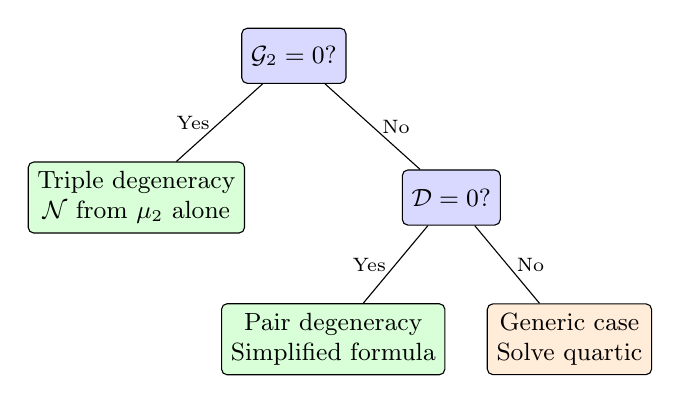
\begin{tikzpicture}[
  level distance=1.8cm,
  level 1/.style={sibling distance=4cm},
  level 2/.style={sibling distance=3cm},
  every node/.style={draw, rectangle, rounded corners=2pt, minimum height=0.7cm, align=center, font=\small},
  decision/.style={fill=blue!15},
  result/.style={fill=green!15},
  compute/.style={fill=orange!15}
]
\node[decision] {$\mathcal{G}_2 = 0$?}
  child {
    node[result] {Triple degeneracy\\$\mathcal{N}$ from $\mu_2$ alone}
    edge from parent node[left,draw=none,font=\scriptsize] {Yes}
  }
  child {
    node[decision] {$\mathcal{D} = 0$?}
    child {
      node[result] {Pair degeneracy\\Simplified formula}
      edge from parent node[left,draw=none,font=\scriptsize] {Yes}
    }
    child {
      node[compute] {Generic case\\Solve quartic}
      edge from parent node[right,draw=none,font=\scriptsize] {No}
    }
    edge from parent node[right,draw=none,font=\scriptsize] {No}
  };
\end{tikzpicture}
\caption{\textbf{Decision tree for negativity computation.} Algebraic conditions $\mathcal{G}_2$ and discriminant $\mathcal{D}$ classify states into branches requiring different computational strategies. Generic states (rightmost branch) require all three moments; degenerate cases admit closed-form solutions.}
\label{fig:decision_tree}
\end{figure}

\paragraph{Multi-copy chirality: entanglement hidden from single-copy measurements on unknown states.}
The chirality correction $C_4 = \mu_4 - I_4$ exposes the first form of hidden entanglement: nonclassical correlations that exist only as patterns \emph{between} multiple copies of a quantum state. Formally, $C_4$ cannot be expressed as $\mathrm{Tr}[O\rho]$ for any single-copy observable $O$---it is an intrinsically multi-copy quantity that requires joint measurements on $\rho^{\otimes 4}$ (Supplementary Section~S4). For a known state reconstructed by full tomography, $C_4$ can of course be computed from the density matrix; the inaccessibility is operational, meaning that no single-copy measurement protocol can extract $C_4$ from an unknown state without first performing complete state reconstruction. These chiral correlations constitute a physically interpretable entanglement signature with a direct geometric meaning (Fig.~\ref{fig:chirality_concept}).

\begin{figure}[t]
\centering
\includegraphics[width=\textwidth]{figure_chirality_3d.pdf}
\caption{\textbf{Multi-copy correlations in the entanglement witness.} \textbf{a}, Computational-basis product states produce coplanar spin patterns with $\chi = 0$. \textbf{b}, Entangled states break coplanarity; the parallelepiped volume equals $\chi \neq 0$. \textbf{c}, Geometric interpretation: solid angle $\omega = 2|\chi|$ on the Bloch sphere. \textbf{d}, Three-spin chirality $\chi_A$: triangular correlations between qubits from three copies of $\rho$. \textbf{e}, Four-copy chirality $\Omega = \tfrac{1}{2}\sum_{i<j<k}\chi_{ijk}$: the symmetric sum over all chirality triples. \textbf{f}, The chirality correction $C_4 = \mu_4 - I_4$; for product states $C_4 = 0$, while entangled states generate $C_4 \neq 0$.}
\label{fig:chirality_concept}
\end{figure}

\textbf{Mathematical structure.} The chirality decomposition has precise algebraic origins. Computing $C_4$ requires comparing four state copies (Fig.~\ref{fig:chirality_concept}d,e), and the underlying operator $\Delta = \sigma^{-1} - \sigma$ decomposes via singlet projectors $P^-_{ij} = \frac{1}{4} - \mathbf{S}_i \cdot \mathbf{S}_j$, where $\mathbf{S}_i$ is the spin operator for qubit $i$. Crucially, the commutators of overlapping projectors yield scalar spin chirality:
\begin{equation}
[P^-_{ij}, P^-_{jk}] = -i\,\chi_{ijk}, \quad \text{where} \quad \chi_{ijk} = \mathbf{S}_i \cdot (\mathbf{S}_j \times \mathbf{S}_k).
\end{equation}
This algebraic structure directly manifests in the moment relations. As derived in Supplementary Section~S3, the operator $\Delta = \sigma^{-1} - \sigma$ governing $C_k = \mu_k - I_k$ decomposes as $\Delta = 4i\,\Omega_k$, where $\Omega_k$ is Hermitian: $\Omega_3 = \chi_{123}$ and $\Omega_4 = \tfrac{1}{2}\sum_{i<j<k}\chi_{ijk}$---the symmetric sum over all four chirality triples on four copies. The products $g_{mn}\chi_{ijk}$ (where $g_{mn} = 2S_{mn} - I$) generate the ``missing'' chirality triples, and imaginary cross-terms cancel identically.

Exploiting the anti-Hermiticity of $\Delta$, the correction takes the manifestly Hermitian correlator form $C_k = 8\,\mathrm{Tr}[\Omega_A\,\Omega_B\;\rho^{\otimes k}]$---a direct correlation of chirality operators on the $A$ and $B$ subsystems. Both chirality factors vanish for product states ($C_k = 0$). For pure states, any entanglement generates non-coplanar chirality configurations with $C_k \neq 0$; for mixed two-qubit separable states, $C_k$ is bounded: $|C_3| \leq 1/36$ and $|C_4| \leq 1/27$ (Supplementary Section~S4).

This decomposition bridges quantum information and condensed matter physics. The scalar spin chirality $\chi_{ijk} = \mathbf{S}_i \cdot (\mathbf{S}_j \times \mathbf{S}_k)$ is the order parameter for chiral spin liquids\cite{KalmeyerLaughlin1987} and drives the topological Hall effect\cite{Taguchi2001}; here, the same operator appears not among physical spins on a lattice, but among correlations spanning \emph{copies} of a bipartite quantum state. The permutation symmetry of the moment relations ensures that all chirality triples contribute equally ($\Omega = \tfrac{1}{2}\sum_{i<j<k}\chi_{ijk}$). Entangled states generate non-coplanar multi-copy spin patterns with finite chirality; product states remain coplanar with $\langle\chi_A\chi_B\rangle = 0$.

\textbf{Geometric interpretation: volume and the correlation tensor.} The chirality correction has a geometric interpretation via the correlation tensor $T_{ij} = \mathrm{Tr}[\rho\,(\sigma_i \otimes \sigma_j)]$, whose columns $\mathbf{T}_x$, $\mathbf{T}_y$, $\mathbf{T}_z$ encode spin--spin correlations. For product states, these three vectors are coplanar, forming a parallelepiped of zero volume: $\det(T) = 0$. For entangled states, the vectors span three-dimensional space with $|\det(T)| > 0$. The key connection is that for all two-qubit states with vanishing local Bloch vectors ($\mathbf{r} = \mathbf{s} = \mathbf{0}$), the chirality correction satisfies $C_4 = \tfrac{3}{4}\det(T)$ exactly (Supplementary Section~S4)---chirality measures the \emph{signed volume} of the correlation parallelepiped, with coefficient $3/4$ fixed by the Bell state value ($\det(T) = -1$, $C_4 = -3/4$). This includes all Bell-diagonal states and their local unitary rotations; for general states with nonzero Bloch vectors, corrections of order $O(|\mathbf{r}|^2 + |\mathbf{s}|^2)$ arise from additional LU invariants (Supplementary Section~S4).

This connects chirality to Bell nonlocality: the CHSH criterion\cite{RevModPhys.81.865} depends on the two largest eigenvalues of $T^{\mathsf{T}}T$, while chirality depends on all three through $\det(T)$. For Bell states, $|\det(T)| = 1$ (maximum volume); the sign distinguishes left- from right-handed correlations.

\paragraph{The chirality--negativity connection.}
Negativity and chirality probe entanglement through complementary mechanisms. Negativity $\mathcal{N}$ detects inseparability through the spectrum of $\rho^{T_A}$; chirality $C_4$ detects it through collective multi-copy interference patterns invisible to any single-copy observable. Both vanish for product states and reach extremal values for Bell states ($\mathcal{N} = 1/2$, $C_4 = -3/4$). For two-qubit pure states $|\psi(\theta)\rangle = \cos(\theta/2)|00\rangle + \sin(\theta/2)|11\rangle$, both are monotonic functions of entanglement:
\begin{equation}
\mathcal{N}(\theta) = \frac{1}{2}\sin\theta, \qquad C_4(\theta) = -\sin^2\theta + \frac{1}{4}\sin^4\theta.
\end{equation}
For two-qubit pure states the relationship simplifies to a compact closed form:
\begin{equation}
-C_4 = 4\mathcal{N}^2(1 - \mathcal{N}^2)
\label{eq:C4_N_relation}
\end{equation}
which can be inverted to yield negativity directly from chirality:
\begin{equation}
\mathcal{N} = \sqrt{\frac{1 - \sqrt{1 + C_4}}{2}}
\label{eq:N_from_C4}
\end{equation}
For pure states, $C_4 = 0$ at the product-state boundary and $C_4 = -3/4$ for maximally entangled Bell states: any pure state with $C_4 \neq 0$ is certified entangled. (Throughout this work, we plot $-C_4$ so that entangled states appear as positive values; in the text, we use the algebraic sign $C_4 \leq 0$.)

For mixed two-qubit separable states, the chirality correction is bounded but non-zero. The tight bounds $|C_3| \leq 1/36$ and $|C_4| \leq 1/27$ are achieved by equal mixtures of three mutually unbiased product states (Supplementary Section~S4):
\begin{equation}
\rho_{\pm} = \tfrac{1}{3}\bigl(|0,0/1\rangle\langle 0,0/1| + |{+},{+/-}\rangle\langle{+},{+/-}| + |y_+,y_{\pm}\rangle\langle y_+,y_{\pm}|\bigr),
\end{equation}
with $C_4(\rho_+) = +1/27$ and $C_4(\rho_-) = -1/27$. This establishes a separation: entangled pure states have $|C_4| \in (0, 3/4]$, while separable states satisfy $|C_4| \leq 1/27 \approx 0.037$---a factor of 20 smaller than the Bell state value. An important limitation: for mixed entangled states, $|C_4|$ can fall below $1/27$, so chirality is a faithful entanglement witness only for pure states. For instance, Werner states $\rho_W = p|\Psi^-\rangle\langle\Psi^-| + (1-p)\mathbb{I}/4$ have $C_4 = -3p^3/4$ (since $\mathbf{r} = \mathbf{s} = \mathbf{0}$ and $\det(T) = -p^3$), so $|C_4|$ exceeds the separable bound only for $p > (4/81)^{1/3} \approx 0.37$. Since entanglement onset is at $p > 1/3 \approx 0.33$, a narrow gap exists where the state is entangled but chirality alone cannot certify it. For mixed states, chirality provides no additional entanglement information beyond what negativity already captures: once all three moments $\{\mu_2, \mu_3, \mu_4\}$ are measured, $C_4 = \mu_4 - I_4$ is fully determined, and negativity from the Newton--Girard reconstruction is the definitive test. The value of chirality lies in its physical interpretation---as a multi-copy handedness correlator---rather than as an independent detection criterion.

The identity $C_k = 8\,\mathrm{Tr}[\Omega_A\,\Omega_B\;\rho^{\otimes k}]$ thus answers the open question of what multi-copy correlations distinguish partial transposition from purity\cite{Bartkiewicz2015moments,PhysRevLett.89.127902,PhysRevLett.90.167901}: they are chirality--chirality correlators, connecting multi-copy entanglement detection to the physics of topological spin systems\cite{KalmeyerLaughlin1987,Taguchi2001}. Remarkably, the same controlled-SWAP circuits that expose this first form of hidden entanglement also reveal a second: bound entangled states, invisible to the entire partial transpose hierarchy, detected through realignment matrix spectral features.

\paragraph{Experimental detection of hidden entanglement.}
We implemented the protocol on IBM Quantum processors using the Heron architecture: IBM Kingston (156 qubits) and IBM Torino (133 qubits). For qubit--qubit ($2 \times 2$) systems, negativity reconstruction from three moments ($\mu_2$, $\mu_3$, $\mu_4$) requires circuits on up to four state copies; for qubit--qutrit ($2 \times 3$), the five moments ($\mu_2, \ldots, \mu_6$) require up to six copies. Figure~\ref{fig:hardware_results}a shows measured versus theoretical negativity for the parametrized family $|\psi(\theta)\rangle$ across both processors and Hilbert space dimensions. Mean errors are 0.002 (Kingston, $2 \times 2$), 0.012 (Torino, $2 \times 2$), and 0.027 (Torino, $2 \times 3$), with statistical uncertainties from $10^5$ shots estimated at $\pm 0.005$ via bootstrap resampling (Supplementary Section~S6). All separable test states ($\theta = 0^\circ$ across both processors and dimensions) yield $\mathcal{N} = 0$ exactly under maximum likelihood calibration, confirming zero false positives within this parametric family. Simulator validation across 37 densely sampled angles confirms negativity accuracy under both ideal conditions (RMSE 0.009) and realistic Torino noise (RMSE 0.044), with zero false positives throughout (Supplementary Fig.~S5a,b). The simulation further validates the protocol on mixed states. Werner states $\rho_W(p)$ correctly show vanishing negativity for $p \leq 1/3$ and monotonically increasing chirality $|C_4|$ with $p$. Bell-product mixtures $\rho_{\mathrm{BP}}(p) = p|\Psi^-\rangle\langle\Psi^-| + (1{-}p)|00\rangle\langle 00|$ confirm entanglement detection for all $p > 0$ (Supplementary Fig.~S5c--f).

\begin{figure}[t]
\centering
\hspace*{-1cm}
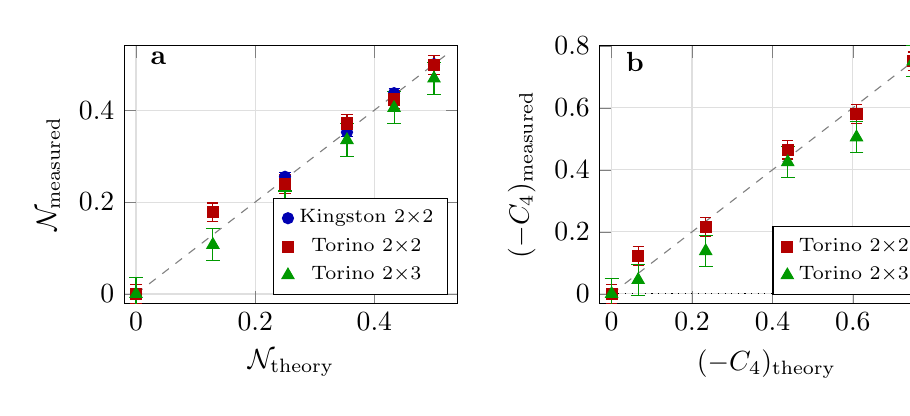
\begin{tikzpicture}
\begin{axis}[
    name=plot1,
    width=0.48\textwidth,
    height=0.4\textwidth,
    xlabel={$\mathcal{N}_{\mathrm{theory}}$},
    ylabel={$\mathcal{N}_{\mathrm{measured}}$},
    xmin=-0.02, xmax=0.54,
    ymin=-0.02, ymax=0.54,
    grid=major,
    grid style={gray!25},
    legend pos=south east,
    legend style={font=\scriptsize},
    title={\textbf{a}},
    title style={at={(0.05,0.95)}, anchor=north west},
]
\addplot[dashed, gray, domain=0:0.52] {x};
\addplot[only marks, mark=*, blue!70!black, mark size=2pt,
    error bars/.cd, y dir=both, y fixed=0.01, error bar style={thin, blue!70!black}]
coordinates {(0.0, 0.0) (0.250, 0.255) (0.354, 0.352) (0.433, 0.437) (0.500, 0.500)};
\addplot[only marks, mark=square*, red!70!black, mark size=2pt,
    error bars/.cd, y dir=both, y fixed=0.02, error bar style={thin, red!70!black}]
coordinates {(0.0, 0.0) (0.129, 0.178) (0.250, 0.239) (0.354, 0.371) (0.433, 0.423) (0.500, 0.498)};
\addplot[only marks, mark=triangle*, green!60!black, mark size=2.5pt,
    error bars/.cd, y dir=both, y fixed=0.035, error bar style={thin, green!60!black}]
coordinates {(0.0, 0.0) (0.129, 0.107) (0.250, 0.189) (0.354, 0.335) (0.433, 0.405) (0.500, 0.469)};
\legend{, Kingston $2{\times}2$, Torino $2{\times}2$, Torino $2{\times}3$}
\end{axis}
\hspace*{1cm}
\begin{axis}[
    at={(plot1.east)},
    anchor=west,
    xshift=0.8cm,
    width=0.48\textwidth,
    height=0.4\textwidth,
    xlabel={$(-C_4)_{\mathrm{theory}}$},
    ylabel={$(-C_4)_{\mathrm{measured}}$},
    xmin=-0.03, xmax=0.80,
    ymin=-0.03, ymax=0.80,
    grid=major,
    grid style={gray!25},
    legend pos=south east,
    legend style={font=\scriptsize},
    title={\textbf{b}},
    title style={at={(0.05,0.95)}, anchor=north west},
]
\addplot[dashed, gray, domain=0:0.78] {x};
\addplot[dotted, black, domain=0:0.78] {0};
\addplot[only marks, mark=square*, red!70!black, mark size=2pt,
    error bars/.cd, y dir=both, y fixed=0.03, error bar style={thin, red!70!black}]
coordinates {(0.0, 0.0) (0.066, 0.122) (0.234, 0.215) (0.438, 0.465) (0.609, 0.580) (0.750, 0.750)};
\addplot[only marks, mark=triangle*, green!60!black, mark size=2.5pt,
    error bars/.cd, y dir=both, y fixed=0.05, error bar style={thin, green!60!black}]
coordinates {(0.0, 0.0) (0.066, 0.045) (0.234, 0.138) (0.438, 0.425) (0.609, 0.505) (0.750, 0.750)};
\legend{, , Torino $2{\times}2$, Torino $2{\times}3$}
\end{axis}
\end{tikzpicture}
\caption{\textbf{Experimental detection of hidden entanglement.} \textbf{a}, Negativity measurements on IBM Quantum processors. Dashed line indicates perfect agreement. For Torino $2\times 2$, the three Bell state measurements are averaged into a single data point at $\mathcal{N} = 0.5$. \textbf{b}, Chirality correction $-C_4 = I_4 - \mu_4$ on IBM Torino (chirality requires four-copy circuits not measured on Kingston). Dotted line marks the product-state value $C_4 = 0$; entangled states yield $C_4 < 0$. Error bars show combined statistical (bootstrap, $10^5$ shots) and systematic (calibration residual) uncertainties, estimated per platform from the root-mean-square deviation of the parametric family.}
\label{fig:hardware_results}
\end{figure}

The maximum likelihood calibration jointly estimates hardware degradation factors and state parameters from a training set with known entanglement (Methods). For Torino, we obtain degradation factor $f_2 = 0.73$ for qubit--qubit systems. Despite hardware degradation, the protocol correctly identifies all entangled states and recovers Bell state properties exactly ($\mathcal{N} = 0.5$, $C_4 = -3/4$).

Figure~\ref{fig:hardware_results}b shows chirality validation, plotting $-C_4 = I_4 - \mu_4$ so that entangled states appear as positive values. The qubit--qutrit system exhibits larger scatter (mean error 0.039 versus 0.022 for qubit--qubit), attributable to the roughly two-fold increase in circuit depth for $2 \times 3$ four-copy circuits. At $10^5$ shots, statistical noise contributes $\lesssim 0.005$ to the negativity error; the residual errors are predominantly systematic (gate and readout), yet all test states are correctly identified as entangled or separable.

\paragraph{Bound entanglement detection.}
The controlled-SWAP infrastructure extends to a second form of hidden entanglement: bound entangled states that possess positive partial transpose (PPT), placing them beyond the reach of \emph{any} criterion based on partial transpose spectra---including the negativity\cite{Horodecki1998bound}, the $p_3$-PPT test\cite{Elben2020mixed}, and the full hierarchy of moment inequalities\cite{Yu2021optimal,Neven2021symmetry}---since the entire PT spectrum is non-negative by definition. Detecting such states requires a mathematically independent criterion. The realignment matrix $R_{(a,a'),(b,b')} = \rho_{(a,b),(a',b')}$\cite{Chen2003,Rudolph2005} provides exactly this: for a $d_A \times d_B$ system, $R$ is a $d_A^2 \times d_B^2$ matrix whose spectral properties are not determined by the PPT condition. Its singular-value moments $\Sigma_k = \mathrm{Tr}[(R^\dagger R)^{k/2}]$ and eigenvalue moments $G_k = \mathrm{Re}\,\mathrm{Tr}[R^k]$ are measurable via the same $k$-copy SWAP test circuits used for chirality detection. For $3 \times 3$ systems ($R$ is $9 \times 9$, with up to nine singular values), even the second-order non-Hermiticity gap $D_2 = \Sigma_2 - G_2$---requiring only two-copy circuits---already separates bound entangled from separable training states. A four-feature SVM classifier based on $D_4 = \Sigma_4 - G_4$, $D_2$, $G_2$, and spectral concentration $\Sigma_2^2/\Sigma_4$ achieves $68/68$ classification accuracy across 27~separable and 41~bound entangled states from three structurally distinct families (Horodecki, Tiles UPB, chessboard) and their noise admixtures, with a false positive rate of $0.038\%$ on $10^5$ random separable states. Hyperparameters ($C = 2000$, $\gamma = 3.0$) were selected by grid search over recall and false positive rate; leave-one-out cross-validation on a 68-state evaluation set confirms 68/68 accuracy (Supplementary Section~S5). Physically, bound entangled states have nearly Hermitian realignment matrices ($D_k \approx 0$) with spread-out singular value spectra (high $\Sigma_2^2/\Sigma_4$), while separable states show substantial non-Hermiticity.

We tested both criteria on IBM quantum hardware using four $3 \times 3$ states: two random separable mixtures and two Horodecki bound entangled states\cite{Horodecki1997} with parameters $a = 0.30$ and $a = 0.70$. Each qutrit was encoded in two physical qubits with $4 \times 10^3$ shots per circuit. The simplified $D_2$ criterion, tested on IBM Fez, correctly classifies all four states with threshold $D_2 = 0.127$ (Fig.~\ref{fig:be_classification}a): separable states yield $D_2 = 0.131$ and $0.184$, while the Horodecki states yield $D_2 = 0.100$ and $0.076$. The two-feature classifier, tested on IBM Marrakesh (Fig.~\ref{fig:be_classification}b; Supplementary Table~S23), likewise identifies all four correctly: separable states exhibit $D_4 = 0.036$ and $0.053$, well above the decision boundary, while the Horodecki states yield $D_4 = 0.006$ ($a = 0.30$) and $D_4 = 2.7 \times 10^{-4}$ ($a = 0.70$), falling below with clear margin. The near-vanishing $D_4$ of the $a = 0.70$ state---three orders of magnitude smaller than separable values---confirms that the near-Hermiticity signature survives realistic hardware noise. Because $D_2$ requires only $O(r^2)$ SWAP-test circuits (16 for $r = 4$ eigenvalues)---a 61-fold reduction over $D_4$---it offers a practical simplified alternative where circuit depth is the primary constraint. Theory-only simulation across 68 states (27 separable, 41 bound entangled---including 25 Horodecki states, Tiles UPB\cite{Bennett1999upb}, and 12 chessboard\cite{Bruss2000chess} parameter sets, plus verified noise admixtures) achieves $68/68$ classification accuracy (Supplementary Fig.~S6).

\begin{figure}[t]
\centering
\begin{minipage}[b]{0.48\textwidth}
\centering
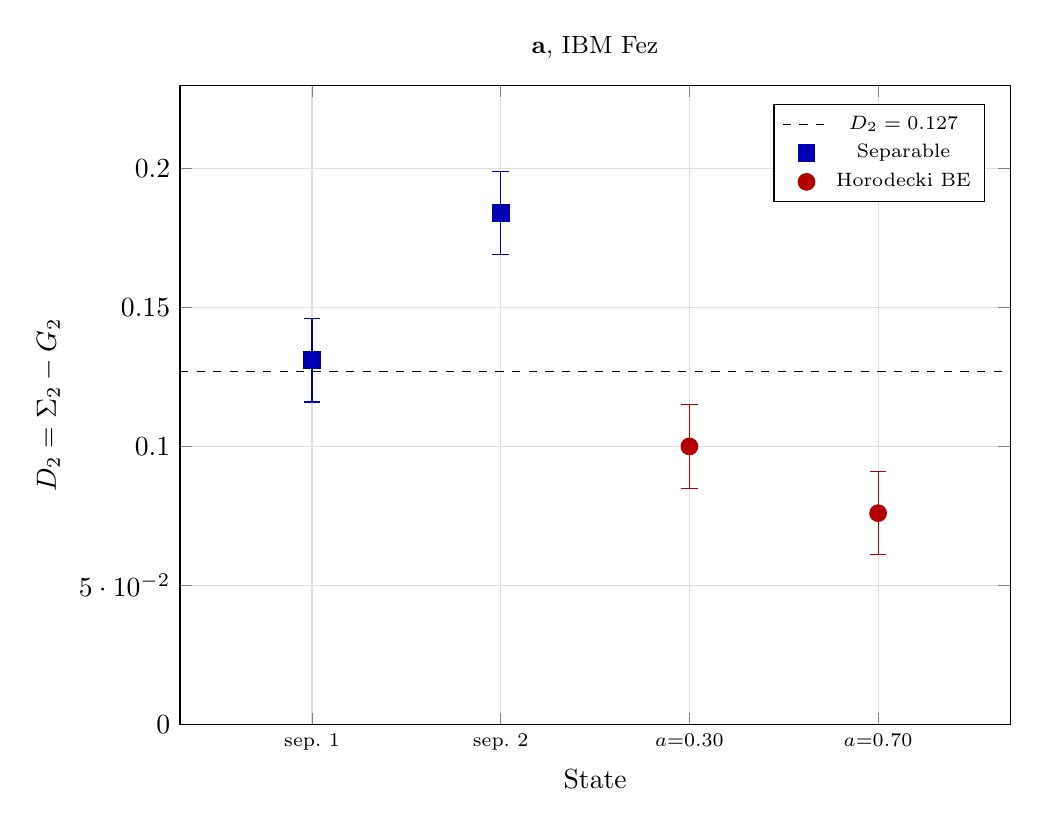
\begin{tikzpicture}
\begin{axis}[
    width=\textwidth,
    height=0.8\textwidth,
    ylabel={$D_2 = \Sigma_2 - G_2$},
    xlabel={State},
    xtick={1,2,3,4},
    xticklabels={sep.~1, sep.~2, {$a{=}0.30$}, {$a{=}0.70$}},
    xticklabel style={font=\scriptsize},
    xmin=0.3, xmax=4.7,
    ymin=0.0, ymax=0.23,
    grid=major,
    grid style={gray!25},
    legend pos=north east,
    legend style={font=\scriptsize},
    title={\textbf{a}, IBM Fez},
    title style={font=\small},
]
% Threshold line
\addplot[dashed, black, domain=0.3:4.7, samples=2] {0.127};
% Separable points (blue squares)
\addplot[only marks, mark=square*, blue!70!black, mark size=3pt,
    error bars/.cd, y dir=both, y fixed=0.015,
    error bar style={thin, blue!70!black}]
coordinates {(1, 0.131) (2, 0.184)};
% Horodecki BE points (red circles)
\addplot[only marks, mark=*, red!70!black, mark size=3pt,
    error bars/.cd, y dir=both, y fixed=0.015,
    error bar style={thin, red!70!black}]
coordinates {(3, 0.100) (4, 0.076)};
\legend{$D_2 = 0.127$, Separable, Horodecki BE}
\end{axis}
\end{tikzpicture}
\end{minipage}
\hfill
\begin{minipage}[b]{0.48\textwidth}
\centering
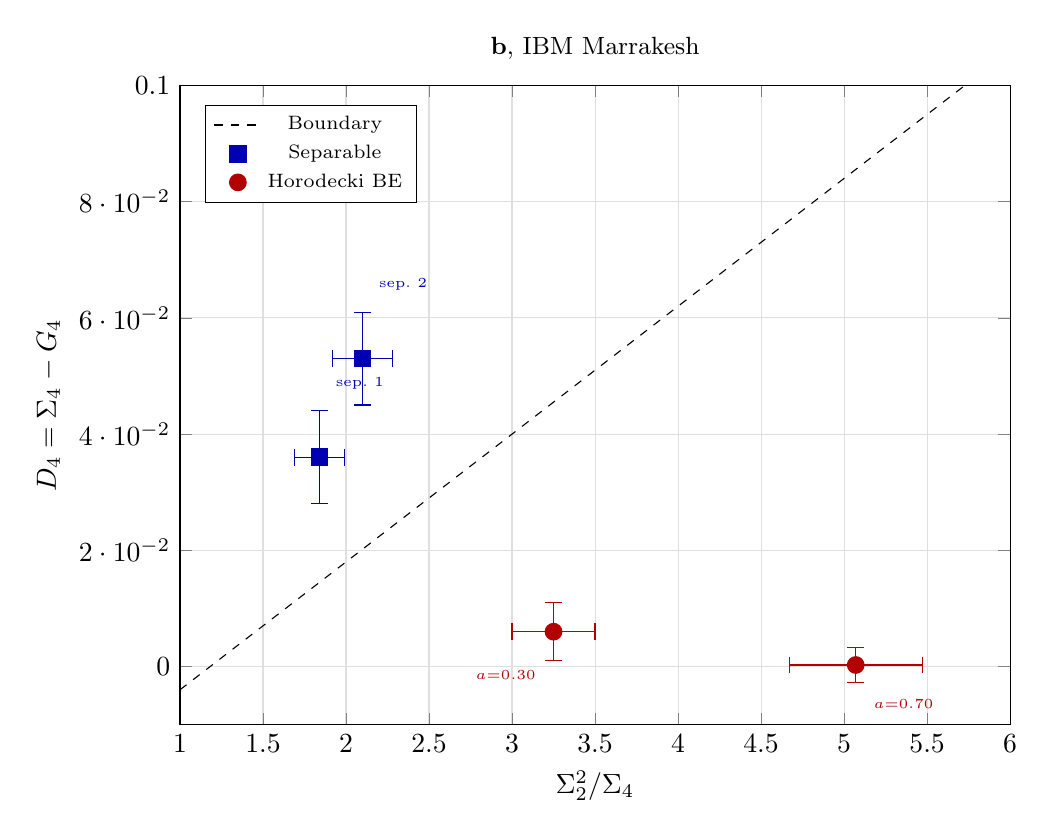
\begin{tikzpicture}
\begin{axis}[
    width=\textwidth,
    height=0.8\textwidth,
    xlabel={$\Sigma_2^2/\Sigma_4$},
    ylabel={$D_4 = \Sigma_4 - G_4$},
    xmin=1.0, xmax=6.0,
    ymin=-0.01, ymax=0.10,
    grid=major,
    grid style={gray!25},
    legend pos=north west,
    legend style={font=\scriptsize},
    title={\textbf{b}, IBM Marrakesh},
    title style={font=\small},
]
\addplot[dashed, black, domain=1.0:6.0, samples=2] {-0.026 + 0.022*x};
\addplot[only marks, mark=square*, blue!70!black, mark size=3pt,
    error bars/.cd, y dir=both, y explicit, x dir=both, x explicit,
    error bar style={thin, blue!70!black}]
coordinates {(1.84, 0.036) +- (0.15, 0.008) (2.10, 0.053) +- (0.18, 0.008)};
\addplot[only marks, mark=*, red!70!black, mark size=3pt,
    error bars/.cd, y dir=both, y explicit, x dir=both, x explicit,
    error bar style={thin, red!70!black}]
coordinates {(3.25, 0.006) +- (0.25, 0.005) (5.07, 0.000271) +- (0.40, 0.003)};
% Point annotations
\node[anchor=south west, font=\tiny, blue!70!black] at (axis cs:1.88, 0.046) {sep.~1};
\node[anchor=south west, font=\tiny, blue!70!black] at (axis cs:2.14, 0.063) {sep.~2};
\node[anchor=north east, font=\tiny, red!70!black] at (axis cs:3.20, 0.001) {$a{=}0.30$};
\node[anchor=north west, font=\tiny, red!70!black] at (axis cs:5.12, -0.004) {$a{=}0.70$};
\legend{Boundary, Separable, Horodecki BE}
\end{axis}
\end{tikzpicture}
\end{minipage}
\caption{\textbf{Bound entanglement detection on IBM quantum hardware.}
\textbf{a},~Simplified one-feature criterion based on the second-order non-Hermiticity gap $D_2 = \Sigma_2 - G_2$ of the realignment matrix, measured on IBM Fez. Dashed line: threshold $D_2 = 0.127$; states below are classified as bound entangled.
\textbf{b},~Two-feature linear classifier in the $(\Sigma_2^2/\Sigma_4,\; D_4)$ plane, measured on IBM Marrakesh. Dashed line: decision boundary $D_4 = -0.026 + 0.022 \cdot (\Sigma_2^2/\Sigma_4)$.
In both panels, blue squares denote random separable mixtures of product states in $\mathbb{C}^3 \otimes \mathbb{C}^3$, and red circles denote Horodecki bound entangled states $\rho_a$~\cite{Horodecki1997} with parameters $a = 0.30$ and $a = 0.70$. Both criteria correctly classify all four states. The $D_2$ criterion requires only $O(r^2)$ SWAP-test circuits (16 for $r=4$ eigenvalues), 61 times fewer than the $D_4$-based classifier. Error bars show $\pm 1\sigma$ shot noise uncertainty from $4 \times 10^3$ shots per circuit.}
\label{fig:be_classification}
\end{figure}

\paragraph{Non-uniform noise characterization.}
Additional controlled-SWAP experiments on IBM Torino---measuring realignment matrix moments for bound entanglement classification\cite{Chen2003,Rudolph2005}---reveal significant state-dependent noise. The degradation factor $f$ varies from 0.61 to 0.92 across quantum states and measurement types, with circuits preparing different input states experiencing up to 50\% attenuation differences for the same target state. This non-uniform degradation is relevant to moment-subtraction strategies: if $\mu_4$ and $I_4$ experience degradation factors $f_{\mu_4}$ and $f_{I_4}$ respectively, the measured chirality correction becomes $C_4^{\mathrm{meas}} = f_{\mu_4}\mu_4 - f_{I_4}I_4$, introducing a bias of $(f_{\mu_4} - f_{I_4})\bar{\mu}_4$ where $\bar{\mu}_4$ is the average moment value. For our Torino data, the fitted per-moment degradation factors differ by $|f_{\mu_4} - f_{I_4}| \lesssim 0.05$, yielding a worst-case chirality bias of $\sim 0.01$---small compared to the entangled-state signal ($|C_4| \geq 0.066$ for $\theta \geq 15^\circ$) but comparable to the separable bound $1/27 \approx 0.037$. The per-moment maximum likelihood calibration employed here absorbs much of this variation, but the finding motivates caution when interpreting uncalibrated moment differences on real hardware.

\paragraph{Efficiency analysis.}
Monte Carlo simulation over $10^5$ Haar-random states confirms that generic two-qubit ($2 \times 2$) states require exactly three moment configurations ($\mu_2, \mu_3, \mu_4$ on two-, three-, and four-copy circuits), yielding $16/3 \approx 5.3\times$ efficiency gain over full tomography in terms of measurement configurations. At $10^5$ shots per configuration, the total shot budget is $3 \times 10^5$ for two-qubit negativity. For qubit--qutrit systems ($2 \times 3$, $d = 6$), five moment configurations ($\mu_2, \ldots, \mu_6$ on up to six-copy circuits) suffice, giving $36/5 \approx 7.2\times$ improvement. Under depolarizing noise $\eta$, the root-mean-square error scales linearly as $\mathrm{RMSE} = (0.245 \pm 0.004)\eta$, remaining below 0.022 for typical NISQ conditions ($\eta < 0.08$). Under depolarizing noise, entanglement is consistently \emph{underestimated}, ensuring the protocol does not falsely report entanglement in separable states within this noise model.

\paragraph{Discussion.}
These results establish that entanglement has a layered structure. The first layer---single-copy properties---is accessible to conventional witnesses and the Peres--Horodecki criterion\cite{PhysRevLett.77.1413,HORODECKI19961,RevModPhys.81.865}. The second layer---multi-copy chirality---requires joint measurements on state replicas to expose collective handedness patterns that no single-copy observable can detect. The third layer---bound entanglement behind the PPT barrier---demands criteria that probe structures independent of the partial transpose spectrum. The controlled-SWAP moment framework provides systematic access to all three layers through shared circuit infrastructure. More generally, a $d_A \times d_B$ system requires $d_A d_B - 1$ independent moments, so the circuit depth (set by the copy number $k$) and the number of configurations both grow linearly in $d_A d_B$---favourable compared to the $O(d^2)$ scaling of full tomography, though the multi-copy overhead per circuit increases accordingly.

The chirality decomposition $C_k = 8\,\mathrm{Tr}[\Omega_A\,\Omega_B\;\rho^{\otimes k}]$ gives physical meaning to the multi-copy correlations probed by partial transpose moments\cite{Bartkiewicz2015moments,PhysRevLett.89.127902,PhysRevLett.90.167901}: the ``handedness'' of spin configurations across state replicas, a collective interference pattern that product states cannot generate. That this takes the mathematical form of scalar spin chirality---the order parameter governing chiral spin liquids and the topological Hall effect\cite{KalmeyerLaughlin1987,Taguchi2001}---is structurally significant: both phenomena probe whether spin vectors span a three-dimensional volume or collapse to a plane. For pure states, $C_4 \neq 0$ certifies entanglement with zero false positives, providing a universal geometric test without prior state knowledge.

The bound entanglement detection addresses a qualitatively harder problem. Previous demonstrations relied on witnesses tailored to specific state families\cite{Amselem2009bound,Zhang2023randomized,Gulati2024ibm}, and all partial-transpose-based criteria\cite{Yu2021optimal,Neven2021symmetry,Lim2011spa} are structurally blind to PPT entangled states. Even the standard realignment criterion---the computable cross-norm (CCNR) condition $\|R(\rho)\|_1 > 1$\cite{Chen2003,Rudolph2005}---which does probe a PPT-independent matrix, detects Horodecki states only for $a \lesssim 0.28$, leaving the majority of the bound entangled parameter range invisible. The realignment non-Hermiticity gap $D_4 = \Sigma_4 - G_4$ overcomes all three limitations: it is state-family-independent, probes a PPT-independent structure, and---through higher-order spectral features---detects Horodecki states across the full range $a \in (0, 1)$, far exceeding the first-order trace-norm criterion. However, one class of criteria remains structurally inaccessible: the range criterion\cite{Horodecki1997}, which tests whether the range of $\rho$ (and of $\rho^{T_A}$) is spanned by product vectors. This condition cannot be expressed as a permutation-trace inequality and thus lies outside the scope of all moment-based protocols. Certain bound entangled states in non-square systems---notably the Horodecki $2 \times 4$ family\cite{DiVincenzo2000}---are detected only by the range criterion and evade both CCNR and the $D_k$ features. For such systems, the spectral framework should be supplemented with range-criterion analysis when full density matrix information is available. That the spectral distinction between bound entangled ($D_4 \sim 10^{-4}$) and separable ($D_4 \sim 10^{-2}$) states persists through hardware noise without classifier recalibration suggests the near-Hermiticity signature is structurally robust. The near-Hermiticity of bound entangled realignment matrices is not merely empirical: for PPT states, the realignment map preserves positivity structure that constrains eigenvalues to approximate singular values, whereas generic separable mixtures---especially those with few product-state terms---develop substantial non-Hermitian character through incoherent averaging (Supplementary Section~S5). The classifier covers all three known $3 \times 3$ PPT entangled families (Horodecki, Tiles UPB, chessboard), their noise admixtures, and cross-family mixtures. Whether exotic constructions in higher dimensions could violate the near-Hermiticity pattern remains an open question that motivates extending the training set as new bound entangled families are discovered.

Compared with prior multi-copy protocols\cite{Bartkiewicz2015moments,Bartkiewicz2017hom,Bartkiewicz2015universal,Lemr2016collectibility,Travnicek2019,tulewicz2025,Elben2020mixed,Huang2020shadows}, the present approach offers two advances: the identification of the specific correlation structure---chirality---encoded in the moment differences $C_k = \mu_k - I_k$, and the extension to bound entanglement via realignment spectral features on the same hardware. Experimentally, the controlled-SWAP test replaces direct singlet projections with a single ancilla measurement, yielding a dimension-independent interface. This is especially significant for qutrits, where the antisymmetric subspace is three-dimensional and no unique singlet exists for projection.

Three limitations deserve emphasis. First, the maximum likelihood calibration relies on states with known entanglement parameters; for truly unknown states, alternative strategies such as reference-state benchmarking would be needed. Perturbation analysis shows the calibration is robust: $\pm 2^\circ$ uncertainty in preparation angles changes the fitted degradation factors by $<1\%$ and the mean negativity error by $<0.003$ (Supplementary Section~S6). Second, the bound entanglement demonstration tests a limited hardware sample (four states per processor); establishing general reliability will require evaluation across broader state families and higher dimensions. The theory-only validation (68 states, three families) and the 0.038\% false positive rate on $10^5$ random separable states provide broader coverage, but the test separable states are generated as Haar-random product-state mixtures with varied ranks (1--81 terms). Structured separable states from specific physical processes could in principle exhibit different feature distributions, though the inclusion of low-rank mixtures (where false positives concentrate) in the test set partially addresses this concern (Supplementary Section~S5). Third, the efficiency comparison of $5.3\times$ (for $2 \times 2$) and $7.2\times$ (for $2 \times 3$) counts measurement configurations but not the qubit overhead of multi-copy circuits: a four-copy two-qubit circuit uses 9 qubits versus 2 for single-copy tomography, though each circuit yields a global scalar rather than a local expectation value.

Nonetheless, the spectral approach requires no prior knowledge of the target state and extends to any bipartite dimension accessible to SWAP-test circuits. The Gr\"obner basis compression to three configurations for two-qubit systems---a five-fold reduction over tomography---is what makes these hidden-entanglement signatures experimentally practical. Compared with classical shadow tomography\cite{Huang2020shadows}, which estimates $k$-th order polynomials of $\rho$ from single-copy randomised bases at a sample cost that grows with the operator complexity, the controlled-SWAP approach uses $O(1)$ circuit configurations per moment with precision scaling as $1/\sqrt{N_{\mathrm{shots}}}$; the trade-off is the need for $k$ coherent state copies per circuit. Looking forward, the framework invites extensions to multipartite systems, higher-order moments, and native gate compilation, with the broader implication that multi-copy spectral methods may reveal further hidden layers in the structure of quantum correlations.

\section*{Methods}

\subsection*{Newton--Girard reconstruction}
For a two-qubit system with partial transpose eigenvalues $\{\lambda_1, \lambda_2, \lambda_3, \lambda_4\}$, the characteristic polynomial $P(x) = x^4 - e_1 x^3 + e_2 x^2 - e_3 x + e_4$ has coefficients related to moments by:
\begin{align}
e_1 &= 1, \quad e_2 = \tfrac{1}{2}(1 - \mu_2), \quad e_3 = \tfrac{1}{6}(1 - 3\mu_2 + 2\mu_3), \nonumber\\
e_4 &= \tfrac{1}{24}(1 - 6\mu_2 + 8\mu_3 + 3\mu_2^2 - 6\mu_4).
\end{align}
Eigenvalues are obtained via Ferrari's method or numerical root-finding; negativity is the sum of absolute values of negative eigenvalues.

\subsection*{Maximum likelihood calibration}
Hardware measurements suffer depth-dependent degradation: $\mu_k^{\mathrm{meas}} = f_k \cdot \mu_k^{\mathrm{ideal}} + \epsilon_k$. Following standard quantum state estimation practice\cite{Hradil1997,Banaszek2000}, we jointly optimize degradation factors $(f_2, f_3, f_4)$ and state parameters $(\theta_1, \ldots, \theta_N)$ by minimizing the negative log-likelihood:
\begin{equation}
-\log \mathcal{L} = \sum_{i,k} \frac{(\mu_k^{\mathrm{meas},i} - f_k \cdot \mu_k^{\mathrm{theo}}(\theta_i))^2}{2\sigma_k^2}.
\end{equation}
For the parametrized family $|\psi(\theta)\rangle = \cos(\theta/2)|00\rangle + \sin(\theta/2)|11\rangle$, theoretical moments are $\mu_2 = 1$, $\mu_3 = \frac{1}{4}(1 + 3\cos^2\theta)$, $\mu_4 = \frac{1}{4}(1 + \cos^2\theta)^2$. The constant $\mu_2 = 1$ for pure states provides a strong calibration constraint. The optimization is performed using L-BFGS-B with bounds $f_k \in [0, 1]$ and $\theta_i \in [0, \pi/2]$. Perturbation analysis (Supplementary Section~S6) shows that the calibration is robust to preparation imperfections: introducing $\pm 2^\circ$ systematic errors in the calibration angles changes the fitted $f_k$ by $<1\%$ and the mean negativity error by $<0.003$. The state-dependent degradation observed on IBM Torino (see Non-uniform noise characterization) suggests that per-state calibration may improve precision beyond the global estimation employed here.

\subsection*{Hardware specifications}
Experiments used IBM Kingston (156 qubits), IBM Torino (133 qubits), IBM Fez (156 qubits), and IBM Marrakesh (156 qubits), all Heron-architecture processors with native gate set \{CZ, $\sqrt{X}$, $R_Z$, $X$\}. Circuits were transpiled using Qiskit optimization level 3 and executed with $10^5$ shots per configuration for negativity and chirality measurements, and $4 \times 10^3$ shots for bound entanglement classification. Readout errors were mitigated using matrix-free measurement mitigation (M3)\cite{Nation2021}.

\subsection*{Test states}

\textit{Negativity and chirality.}
We test parametrised pure states $|\psi(\theta)\rangle = \cos(\theta/2)|00\rangle + \sin(\theta/2)|11\rangle$ with $\theta \in [0^\circ, 90^\circ]$ spanning the full range from product to maximally entangled. Simulator validation additionally uses Werner states $\rho_W(p) = p|\Psi^-\rangle\langle\Psi^-| + (1-p)\mathbb{I}/4$ (entangled for $p > 1/3$) and Bell-product mixtures $\rho_{\mathrm{BP}}(p) = p|\Psi^-\rangle\langle\Psi^-| + (1-p)|00\rangle\langle 00|$ (entangled for all $p > 0$).

\textit{Bound entanglement.}
We test three structurally distinct families of PPT entangled states in $\mathbb{C}^3 \otimes \mathbb{C}^3$: Horodecki states\cite{Horodecki1997} ($a \in \{0.10, \ldots, 0.90\}$, the prototypical bound entangled family), Tiles UPB states\cite{Bennett1999upb} (constructed from unextendible product bases), and chessboard states\cite{Bruss2000chess} (rank-4 states with checkerboard zero pattern, entangled when $cmn \neq abc$). Random separable states are mixtures of Haar-random product states. Explicit constructions and parameter sets are given in Supplementary Section~S5.

\subsection*{Data availability}
Raw measurement data and analysis code are available at \url{https://github.com/barkol/grobner-negativity} and will be deposited on Zenodo upon publication.

\section*{Acknowledgements}
P.T. and K.B. are supported by the Polish National Science Centre (Maestro Grant No. DEC-2019/34/A/ST2/00081).

\section*{Author contributions}
P.T. developed the theoretical framework, implemented circuits, and performed experiments. K.B. conceived the project and supervised the research. Both authors wrote the manuscript.

\section*{Competing interests}
The authors declare no competing interests.

\begin{thebibliography}{40}

\bibitem{RevModPhys.81.865}
Horodecki, R., Horodecki, P., Horodecki, M. \& Horodecki, K. Quantum entanglement. \textit{Rev. Mod. Phys.} \textbf{81}, 865--942 (2009).

\bibitem{Huang2020shadows}
Huang, H.-Y., Kueng, R. \& Preskill, J. Predicting many properties of a quantum system from very few measurements. \textit{Nat. Phys.} \textbf{16}, 1050--1057 (2020).

\bibitem{Elben2020mixed}
Elben, A. \textit{et al.} Mixed-state entanglement from local randomized measurements. \textit{Phys. Rev. Lett.} \textbf{125}, 200501 (2020).

\bibitem{PhysRevLett.77.1413}
Peres, A. Separability criterion for density matrices. \textit{Phys. Rev. Lett.} \textbf{77}, 1413--1415 (1996).

\bibitem{HORODECKI19961}
Horodecki, M., Horodecki, P. \& Horodecki, R. Separability of mixed states: necessary and sufficient conditions. \textit{Phys. Lett. A} \textbf{223}, 1--8 (1996).

\bibitem{KalmeyerLaughlin1987}
Kalmeyer, V. \& Laughlin, R. B. Equivalence of the resonating-valence-bond and fractional quantum Hall states. \textit{Phys. Rev. Lett.} \textbf{59}, 2095--2098 (1987).

\bibitem{Taguchi2001}
Taguchi, Y. \textit{et al.} Spin chirality, Berry phase, and anomalous Hall effect in a frustrated ferromagnet. \textit{Science} \textbf{291}, 2573--2576 (2001).

\bibitem{Nation2021}
Nation, P. D., Kang, H., Sundaresan, N. \& Gambetta, J. M. Scalable mitigation of measurement errors on quantum computers. \textit{PRX Quantum} \textbf{2}, 040326 (2021).

\bibitem{PhysRevLett.89.127902}
Horodecki, P. \& Ekert, A. Method for direct detection of quantum entanglement. \textit{Phys. Rev. Lett.} \textbf{89}, 127902 (2002).

\bibitem{PhysRevLett.90.167901}
Horodecki, P. Measuring quantum entanglement without prior state reconstruction. \textit{Phys. Rev. Lett.} \textbf{90}, 167901 (2003).

\bibitem{tulewicz2025}
Tulewicz, P., Bartkiewicz, K., Miranowicz, A. \& Nori, F. Resource-efficient quantum correlation measurements via multicopy neural network methods. \textit{Sci. Rep.} \textbf{15}, 40868 (2025).

\bibitem{Travnicek2019}
Tr\'avn\'{\i}\v{c}ek, V., Bartkiewicz, K., \v{C}ernoch, A. \& Lemr, K. Experimental measurement of the Hilbert-Schmidt distance between two-qubit states. \textit{Phys. Rev. Lett.} \textbf{123}, 260501 (2019).

\bibitem{Hradil1997}
Hradil, Z. Quantum-state estimation. \textit{Phys. Rev. A} \textbf{55}, R1561--R1564 (1997).

\bibitem{Banaszek2000}
Banaszek, K., D'Ariano, G. M., Paris, M. G. A. \& Sacchi, M. F. Maximum-likelihood estimation of the density matrix. \textit{Phys. Rev. A} \textbf{61}, 010304(R) (2000).

\bibitem{Chen2003}
Chen, K. \& Wu, L.-A. A matrix realignment criterion for recognizing entanglement. \textit{Quant. Inf. Comput.} \textbf{3}, 193--202 (2003).

\bibitem{Rudolph2005}
Rudolph, O. Further results on the cross norm criterion for separability. \textit{Quant. Inf. Process.} \textbf{4}, 219--239 (2005).

\bibitem{Horodecki1998bound}
Horodecki, M., Horodecki, P. \& Horodecki, R. Mixed-state entanglement and distillation: Is there a ``bound'' entanglement in nature? \textit{Phys. Rev. Lett.} \textbf{80}, 5239--5242 (1998).

\bibitem{Horodecki1997}
Horodecki, P. Separability criterion and inseparable mixed states with positive partial transposition. \textit{Phys. Lett. A} \textbf{232}, 333--339 (1997).

\bibitem{Bartkiewicz2015moments}
Bartkiewicz, K., Beran, J., Lemr, K., Norek, M. \& Miranowicz, A. Quantifying entanglement of a two-qubit system via measurable and invariant moments of its partially transposed density matrix. \textit{Phys. Rev. A} \textbf{91}, 022323 (2015).

\bibitem{Bartkiewicz2017hom}
Bartkiewicz, K., Chimczak, G. \& Lemr, K. Direct method for measuring and witnessing quantum entanglement of arbitrary two-qubit states through Hong-Ou-Mandel interference. \textit{Phys. Rev. A} \textbf{95}, 022331 (2017).

\bibitem{Yu2021optimal}
Yu, X.-D., Imai, S. \& G\"uhne, O. Optimal entanglement certification from moments of the partial transpose. \textit{Phys. Rev. Lett.} \textbf{127}, 060504 (2021).

\bibitem{Neven2021symmetry}
Neven, A. \textit{et al.} Symmetry-resolved entanglement detection using partial transpose moments. \textit{npj Quantum Inf.} \textbf{7}, 152 (2021).

\bibitem{Lemr2016collectibility}
Lemr, K., Bartkiewicz, K. \& \v{C}ernoch, A. Experimental measurement of collective nonlinear entanglement witness for two qubits. \textit{Phys. Rev. A} \textbf{94}, 052334 (2016).

\bibitem{Lim2011spa}
Lim, H.-T., Kim, Y.-S., Ra, Y.-S., Bae, J. \& Kim, Y.-H. Experimental realization of an approximate partial transpose for photonic two-qubit systems. \textit{Phys. Rev. Lett.} \textbf{107}, 160401 (2011).

\bibitem{Bartkiewicz2015universal}
Bartkiewicz, K., Horodecki, P., Lemr, K., Miranowicz, A. \& \.Zyczkowski, K. Method for universal detection of two-photon polarization entanglement. \textit{Phys. Rev. A} \textbf{91}, 032315 (2015).

\bibitem{Amselem2009bound}
Amselem, E. \& Bourennane, M. Experimental four-qubit bound entanglement. \textit{Nat. Phys.} \textbf{5}, 748--752 (2009).

\bibitem{Zhang2023randomized}
Zhang, C. \textit{et al.} Experimental verification of bound and multiparticle entanglement with the randomized measurement toolbox. Preprint at \url{https://arxiv.org/abs/2307.04382} (2023).

\bibitem{Gulati2024ibm}
Gulati, V., Singh, G. \& Dorai, K. Using linear and nonlinear entanglement witnesses to generate and detect bound entangled states on an IBM quantum processor. \textit{Phys. Scr.} \textbf{99}, 095112 (2024).

\bibitem{Bennett1999upb}
Bennett, C. H. \textit{et al.} Unextendible product bases and bound entanglement. \textit{Phys. Rev. Lett.} \textbf{82}, 5385--5388 (1999).

\bibitem{Bruss2000chess}
Bru\ss, D. \& Peres, A. Construction of quantum states with bound entanglement. \textit{Phys. Rev. A} \textbf{61}, 030301(R) (2000).

\bibitem{DiVincenzo2000}
DiVincenzo, D. P. \textit{et al.} Evidence for bound entangled states with negative partial transpose. \textit{Phys. Rev. A} \textbf{61}, 062312 (2000).

\end{thebibliography}


\end{document}
